\synctex=1
\documentclass[12pt]{article}
% Import geometry for smaller top
\usepackage{geometry}
% Required for inserting images
\usepackage{graphicx}
\graphicspath{{./images/}}
% Header and footer
\usepackage{fancyhdr}
% Language setting
\usepackage[utf8]{inputenc}
\usepackage[T2A]{fontenc}
\usepackage[russian]{babel}
% For better list
\usepackage{enumitem}
% For correct math operation
\usepackage{amsmath}
\usepackage{hyperref}
\usepackage{multirow}

\geometry{a4paper,
 total={170mm,257mm},
 left=20mm,
 top=30mm,
 bottom=25mm
}

\fancypagestyle{first style}
{
\chead{\footnotesize{Санкт-Петербургский Национальный Исследовательский Университет ИТМО\\Факультет Технологического Менеджмента и Инноваций}}
\cfoot{\footnotesize{Санкт-Петербург 2025г.}}
\renewcommand{\headrulewidth}{0pt}
}

\begin{document}

\pagestyle{fancy}
\thispagestyle{first style}

\centering{
\includegraphics[scale=0.5]{LogoITMO}}

\vspace{25mm}

\centering{Вариант №14\\Лабораторная Работа №4\\По дисциплине\\Вычислительная математика}

\vspace{50mm}

\begin{flushright}
Выполнил студент группы P3218:\\Хромов Даниил Тимофеевич\\
\vspace{5mm}
Преподаватель:\\Бострикова Дарья Константиновна\\
\end{flushright}

\newpage

\pagestyle{empty}
\raggedright

\textit{Цель работы:} решить задачу интерполяции, найти значения функции при заданных значениях аргумента, отличных от узловых точек.\\

\section{Вычислительная реализация задачи}

\subsection{Выбрать таблицу $y = f(x)$}
\begin{center}
\begin{tabular}{|c|c|c|c|c|c|}
  \hline
  \multicolumn{1}{|c|}{} & x & y & № варианта & $X_1$ & $X_2$ \\
  \hline
  \multirow{7}{*}{Таблица 1.4} 
  & 1.05 & 0.1213 & \multirow{7}{*}{14} & \multirow{7}{*}{1.112} & \multirow{7}{*}{1.319} \\
  & 1.15 & 1.1316 & & & \\
  & 1.25 & 2.1459 & & & \\
  & 1.35 & 3.1565 & & & \\
  & 1.45 & 4.1571 & & & \\
  & 1.55 & 5.1819 & & & \\
  & 1.65 & 6.1969 & & & \\
  \hline
\end{tabular}
\end{center}

\subsection{Построить таблицу конечных разностей}
\begin{center}
\begin{tabular}{|c|c|c|c|c|c|c|c|c|}
  \hline
  № & $x_i$ & $y_i$ & $\Delta y_i$ & $\Delta^2 y_i$ & $\Delta^3 y_i$ & $\Delta^4 y_i$ & $\Delta^5 y_i$ & $\Delta^6 y_i$ \\
  \hline
  0 & 1.05 & 0.1213 & 1.0103 & 0.0040 & -0.0077 & 0.0014 & 0.0391 & -0.1478 \\
  1 & 1.15 & 1.1316 & 1.0143 & -0.0037 & 0.0063 & 0.0405 & -0.1087 & \\
  2 & 1.25 & 2.1459 & 1.0106 & -0.0100 & 0.0342 & -0.0682 & & \\
  3 & 1.35 & 3.1565 & 1.0006 & 0.0242 & -0.0340 & & & \\
  4 & 1.45 & 4.1571 & 1.0248 & -0.0098 & & & & \\
  5 & 1.55 & 5.1819 & 1.0150 & & & & & \\
  6 & 1.65 & 6.1969 & & & & & & \\
  \hline
\end{tabular}
\end{center}

\subsection{Вычислить значения функции для аргумента $X_1$}
\textbf{Уточнение:} Используя первую или вторую интерполяционную формулу Ньютона:\\
\vspace{5mm}
Воспользуемся формулой Ньютона для интерполирования \textbf{вперед}, так как $X_1 = 1,112$ лежит в левой половине отрезка.\\
\vspace{5mm}
Для $X_1 = 1,112: \ t = \frac{(x-x_n)}{h} = \frac{1,112-1,05}{0,1} = 0,62 $\\
\vspace{5mm}
$$N_6(x) = y_0 + t\Delta y_0 + \frac{t(t-1)}{2!} \Delta^2 y_0 + \frac{t(t-1)(t-2)}{3!} \Delta^3 y_0 + \frac{t(t-1)(t-2)(t-3)}{4!} \Delta^4 y_0 + $$
$$ + \frac{t(t-1)(t-2)(t-3)(t-4)}{5!} \Delta^5 y_0 + \frac{t(t-1)(t-2)(t-3)(t-4)(t-5)}{6!} \Delta^6 y_0 $$

$$ y(1,112) \approx 0,1213 + 0,62*1,0103 + \frac{0,62(0,62 - 1)}{2} * 0,004 + \frac{0,62(0,62-1)(0,62-2)}{6}*(-0,0077) + $$
$$ + \frac{0,62(0,62-1)(0,62-2)(0,62-3)}{24} * 0,0014 + \frac{0,62(0,62-1)(0,62-2)(0,62-3)(0,62-4)}{120} * 0,0391 + $$
$$ + \frac{0,62(0,62-1)(0,62-2)(0,62-3)(0,62-4)(0,62-5)}{720} * (-0,1478) $$

\vspace{5mm}
$y(1,112) \approx 0,7459$

\subsection{Вычислить значения функции для аргумента $X_2$}
\textbf{Уточнение:} используя первую или вторую интерполяционную формулу Гаусса:\\
\vspace{5mm}
Центральная точка $\alpha = 1,35$, $X_2 = 1,319 < 1,35$, то есть $x<a \rightarrow $ используем вторую интерполяционную формулу Гаусса:\\
\vspace{5mm}
$ t = \frac{(x-x_0)}{h} = \frac{1,319 - 1,35}{0,1} = -0,31 $\\
\vspace{5mm}
$$P_6(x) = y_0 + t\Delta y_{-1} + \frac{t(t-1)}{2!} \Delta^2 y_{-1} + \frac{t(t-1)(t-2)}{3!} \Delta^3 y_{-1} + \frac{t(t-1)(t-2)(t-3)}{4!} \Delta^4 y_{-1} + $$
$$ + \frac{t(t-1)(t-2)(t-3)(t-4)}{5!} \Delta^5 y_{-1} + \frac{t(t-1)(t-2)(t-3)(t-4)(t-5)}{6!} \Delta^6 y_{-1} $$

$$ y(1,319) \approx 3,1565 + 0,62*1,0106 + \frac{0,62(0,62 - 1)}{2} * (-0,01) + \frac{0,62(0,62-1)(0,62-2)}{6}*(0,0063) + $$
$$ + \frac{0,62(0,62-1)(0,62-2)(0,62-3)}{24} * 0,0405 + \frac{0,62(0,62-1)(0,62-2)(0,62-3)(0,62-4)}{120} * 0,0391 + $$
$$ + \frac{0,62(0,62-1)(0,62-2)(0,62-3)(0,62-4)(0,62-5)}{720} * (-0,1478) $$
\vspace{5mm}
$$ y(1,319) \approx 3,7865 $$

\newpage
\section{Программная реализация задачи}
\vspace{5mm}
\url{https://github.com/Ran4er/mystudy/tree/main/4%20computMath/lab_5}\\
\vspace{5mm}
Результаты выполнения программы для различных исходных данных:\\
\fbox{\begin{minipage}{42em}
$\Delta^0$: [0.000000, 1.000000, 2.000000, 3.000000, 4.000000]\\
$\Delta^1$: [1.000000, 1.000000, 1.000000, 1.000000]\\
$\Delta^2$: [0.000000, 0.000000, 0.000000]\\
$\Delta^3$: [0.000000, 0.000000]\\
$\Delta^4$: [0.000000]\\
\\
Lagrange: 3.000000\\
Newton: 3.000000\\
Gauss: 3.000000
\end{minipage}}\\
\vspace{5mm}
\centering
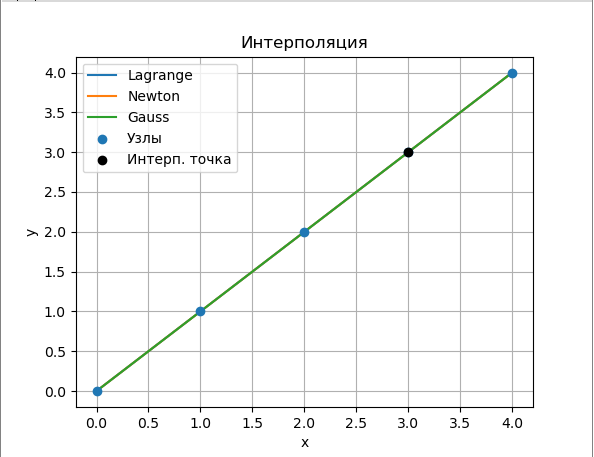
\includegraphics[scale=0.7]{interpolation_pict.png}\\
(Рис. 1. График интерполяции для некоторого набора тестовых узлов)\\
\raggedright

\section*{Вывод}

В ходе выполнения данной лабораторной работы я рассмотрел и реализовал методы интерполяции Ньютона и Гаусса для заданной таблицы данных. Интерполяция позволяет нам предсказывать значения функции в промежуточных точках на основе имеющихся данных.
С помощью разработанной программы были вычислены приближенные значения функции для заданных аргументов с использованием методов Ньютона и Гаусса. Было проведено сравнение результатов, полученных разными методами.
Результаты показали, что оба метода могут быть эффективно использованы для интерполяции, но их точность может зависеть от конкретной функции и распределения данных. Эта работа подчеркивает важность выбора подходящего метода интерполяции в соответствии с требованиями конкретной задачи.

\end{document}
